% 探索（再実施）：確定した設定でのルールベース3手法の検証（親：W001。問いは未確定）
% ファイル名とフォルダ名の番号づけは，タスク T005 が行う
% コンパイル：uplatex を2回 → dvipdfmx（TEXINPUTS で .claude/templates/progress_report// を参照）
\documentclass[twocolumn, 10pt]{ujarticle}
\usepackage{progress_report}

\begin{document}

\reportid{番号未定}
\questionid{W001}
\exploration{ベースラインの設定で，ルールベースの入札手法はどう動くか}
\reportdate{20261010}
\summary{%
REP001で決めたベースラインの設定（3手法とも本家の既定値）で，ルールベースの入札手法（PID，ABid，Online LP）をシミュレータで動かし，以後の比較の基準になる値を記録した。
広告主48社の位置×4エピソード（192セル）で比べたところ，144 runがすべて完走し，scoreの合計はOnline LPが最大で，ABidを1.0としてOnline LP 1.51，PID 0.78であった。
実績CPAが制約を超えたセルの割合は，PID 0.82，ABid 0.85，Online LP 0.39であった。1 runは約2〜3分・約2.9GBで，再実行の結果は完全に一致した。
}
\beginverification

% ============================================================
\section{目的}\label{sec:e-purpose}
% ============================================================

REP001で決めたベースラインの設定で，ルールベースの入札手法（PID，ABid，Online LP）がこのシミュレータでどう動くかを知り，以後の比較の基準になる値を作る。

% ============================================================
\section{実験}\label{sec:e-exp}
% ============================================================

\subsection{対象のアルゴリズム}\label{sec:e-algo}

3手法とも，各ティックの頭に，広告機会（PV）ごとの入札額を「$\alpha\times$価値」で決める（価値は購入確率）。
違いは，入札係数$\alpha$の決め方である（表\ref{tab:algo}）。

\begin{table}[H]
\centering
\caption{3手法の$\alpha$の決め方（数値は既定値）}
\label{tab:algo}
\footnotesize
\begin{tabularx}{\linewidth}{@{}l>{\raggedright\arraybackslash}p{0.2\linewidth}>{\raggedright\arraybackslash}X@{}}
\toprule
手法 & 見るもの & $\alpha$の決め方 \\
\midrule
PID & 残り予算，前のティックの支払い & 最初は15。今のペースで使い切る量が残り予算の0.7倍未満なら1.2倍，1.1倍超なら0.7倍 \\
\addlinespace
ABid & CPA制約，今のティックの価値 & CPA制約$\times$（価値$\div$価値の平均）。価値が高いPVほど強気。予算は見ない \\
\addlinespace
Online LP & 残り予算，早見表，CPA制約 & 過去の1日の記録で，割安なPVから順に買ったとき，残り予算で買える境目の値段。上限はCPA制約の1.5倍 \\
\bottomrule
\end{tabularx}
\end{table}

% 2段抜きの図は，2ページ目の上に出すためにここで宣言する
\begin{figure*}[t]
\centering
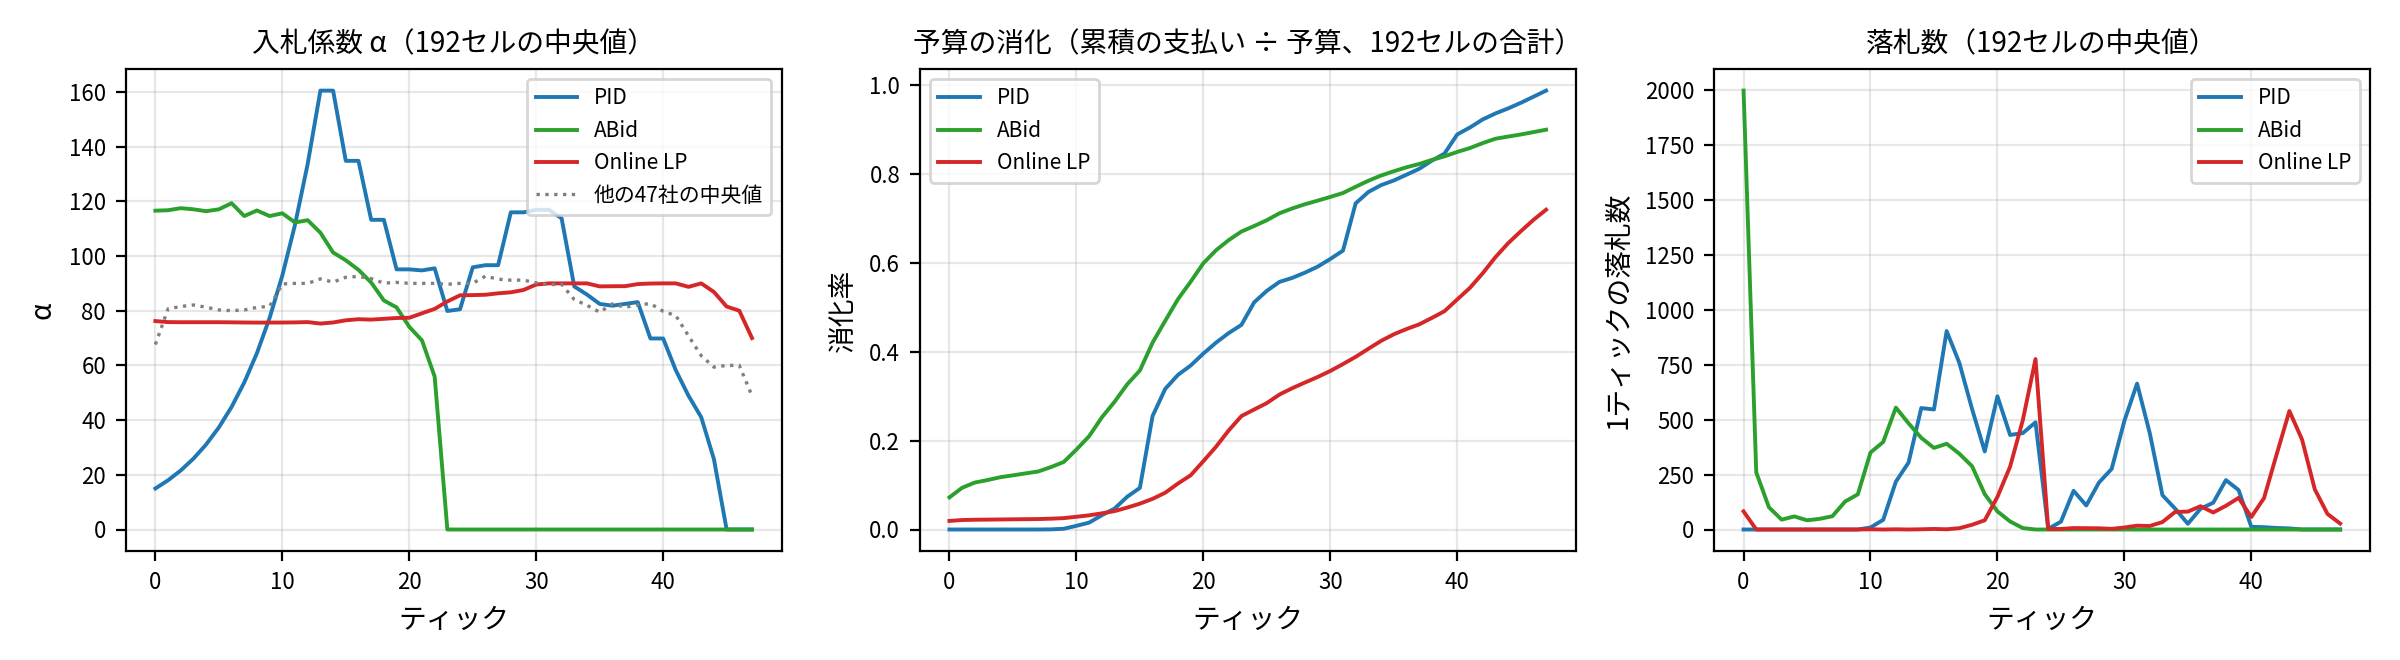
\includegraphics[width=0.8\textwidth]{fig/fig_alpha_time.png}
\caption{3手法の時系列。左：実効の入札係数$\alpha$（192セルの中央値。点線は他の47社の中央値），中：予算の消化（累積の支払い$\div$予算），右：落札数（192セルの中央値）}
\label{fig:alpha}
\end{figure*}
\begin{figure*}[t]
\centering
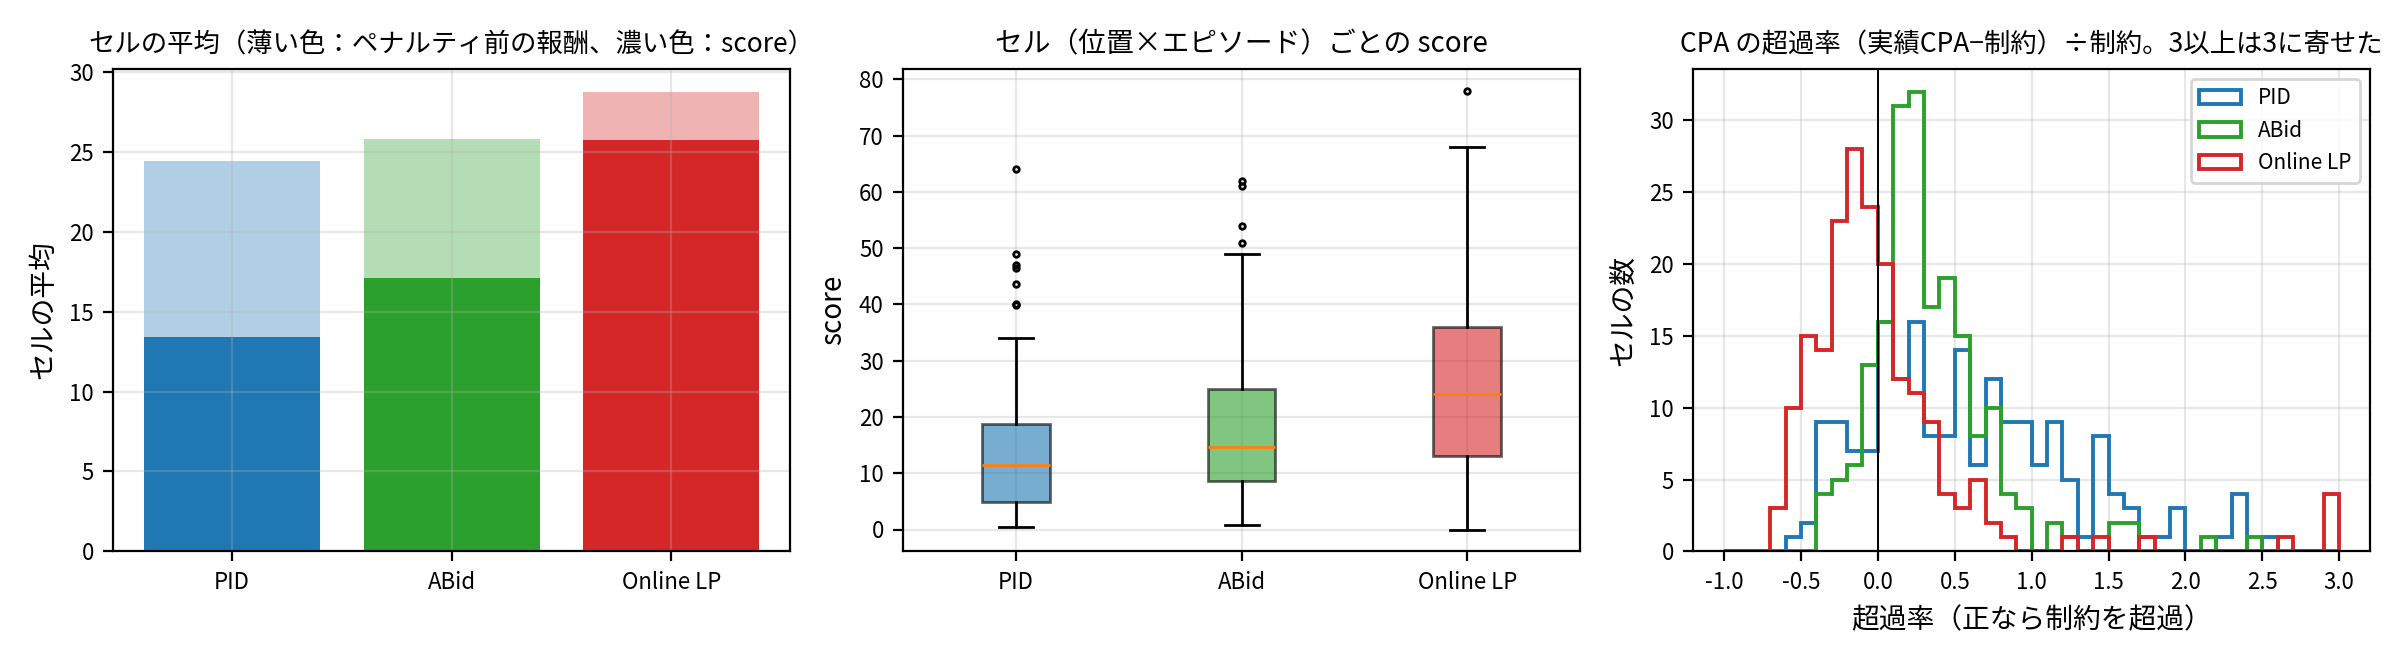
\includegraphics[width=0.8\textwidth]{fig/fig_scores.png}
\caption{3手法の成績とCPA。左：セルの平均（薄い色はペナルティ前の報酬，濃い色はscore），中：セルごとのscore，右：CPAの超過率の分布（正なら制約を超過）}
\label{fig:scores}
\end{figure*}

\subsection{実験環境}\label{sec:e-env}

48社のうち1社（プレイヤー）を対象の手法に差し替え，残りの47社は環境に同梱の手法のままにした（表\ref{tab:cond}）。
成績は，エピソードごとの「購入数$\times$ペナルティ係数」（以下，score）で見る。
ペナルティ係数は，実績CPAが制約を超えたときだけ（制約$\div$実績CPA）$^2$になり，超えなければ1である。
CPAの超過率は，（実績CPA$-$制約）$\div$制約とする。

\begin{table}[H]
\centering
\caption{実験の条件（1 run$=$1位置$\times$4エピソード，1セル$=$1位置$\times$1エピソード）}
\label{tab:cond}
\footnotesize
\begin{tabularx}{\linewidth}{@{}l>{\raggedright\arraybackslash}X@{}}
\toprule
固定 & シミュレータは既定の設定，乱数seed=1 \\
 & 3手法のパラメータは既定値（REP001で決めた設定） \\
 & Linux，Python 3.9.16，CPU。同じ端末・同じコードの版 \\
\midrule
比較 & 3手法 \\
 & 位置48$\times$エピソード0〜3（192セル） \\
 & 計144 run \\
\midrule
再現性 & PID・位置0・エピソード0〜3を再実行（1 run） \\
\bottomrule
\end{tabularx}
\end{table}

\subsection{取った特徴量}\label{sec:e-feat}

成績のほかに，あとから原因を考えるための量を，ティックごとに記録した（表\ref{tab:feat}）。

\begin{table}[H]
\centering
\caption{取った特徴量}
\label{tab:feat}
\footnotesize
\begin{tabularx}{\linewidth}{@{}l>{\raggedright\arraybackslash}X@{}}
\toprule
種類 & 記録した量 \\
\midrule
入札の強さ & 実効の$\alpha$（入札額の和$\div$価値の和），その順位，他47社の$\alpha$の中央値 \\
市場 & 最低落札価格，予算が残る広告主の数，全体の支出 \\
予算のペース & 支払い，残り予算，PV数，予算消化率，最後に落札したティック \\
落札の中身 & 落札数（スロット別），露出数，価値の平均とばらつき \\
CPA & 実績CPA，超過率，ペナルティ係数，ペナルティ前の購入数 \\
位置と他社 & 予算，CPA制約，カテゴリ，全48社の成績と順位 \\
規模 & 所要時間（全体，\texttt{bidding()}1回），最大メモリ \\
\bottomrule
\end{tabularx}
\end{table}

% ============================================================
\section{結果}\label{sec:e-result}
% ============================================================

\textbf{動作}　144 run（3手法$\times$48位置）が，すべて完走し，scoreは有限であった。

\textbf{規模感と再現性}　1 run（7〜8並列）の平均は，PID 163秒，ABid 162秒，Online LP 152秒で，最大メモリは約2.9GBであった（3並列では121〜148秒）。
\texttt{bidding()}1回は，平均0.13ms，0.26ms，1.63ms，最大でも3.64msであった。
同じ設定の再実行で，エピソード・ティック・広告主ごとの記録の全列（時間とメモリを除く）が，完全に一致した（差は0.0）。

\textbf{3手法の比較}　表\ref{tab:cmp}と図\ref{fig:scores}のとおり，scoreの合計は，Online LP，ABid，PIDの順で，Online LPはPIDの1.92倍，ABidの1.51倍であった。
セル単位でOnline LPがPIDを上回った割合は0.77，ABidを上回った割合は0.69，ABidがPIDを上回った割合は0.57であった。
6カテゴリごと，4エピソードごとの合計は，すべてOnline LPが最大であった。
論文の「Online LPが最良」とは同じ向きである。ただし，論文の図10（目視の概算）は，ABidを1.0としてOnline LP 6.5〜7，PID 2.3〜3.5であり，倍率と，PIDとABidの順序は合っていない（原因は確かめていない）。

\begin{table}[H]
\centering
\caption{3手法の比較（192セル）}
\label{tab:cmp}
\footnotesize
\begin{tabularx}{\linewidth}{@{}Xrrr@{}}
\toprule
 & PID & ABid & Online LP \\
\midrule
scoreの合計 & 2,570 & 3,279 & 4,936 \\
ABidを1.0とした値 & 0.78 & 1.00 & 1.51 \\
セルの平均score & 13.4 & 17.1 & 25.7 \\
ペナルティ前の平均報酬 & 24.4 & 25.8 & 28.8 \\
ペナルティ係数の平均 & 0.53 & 0.63 & 0.85 \\
予算消化率の平均 & 0.99 & 0.93 & 0.75 \\
順位の中央値（48社中） & 35 & 32 & 18 \\
\bottomrule
\end{tabularx}
\end{table}

\textbf{CPA制約の達成状況}　表\ref{tab:cpa}のとおり，実績CPAが制約を超えたセルの割合は，PID 0.82，ABid 0.85，Online LP 0.39であった。

\begin{table}[H]
\centering
\caption{CPA制約の達成状況（192セル）}
\label{tab:cpa}
\footnotesize
\begin{tabularx}{\linewidth}{@{}Xrrr@{}}
\toprule
 & PID & ABid & Online LP \\
\midrule
制約を超えたセルの割合 & 0.82 & 0.85 & 0.39 \\
超過率の中央値 & $+0.51$ & $+0.24$ & $-0.09$ \\
超過率が0.5を超えたセルの数 & 97 & 49 & 19 \\
ペナルティで失った報酬の割合 & 0.45 & 0.34 & 0.11 \\
\bottomrule
\end{tabularx}
\end{table}

\textbf{$\alpha$の時間変化}　図\ref{fig:alpha}のとおり，PIDは，ティック0の$\alpha$が15で（他47社の中央値は68），落札数の中央値が0を超えるのはティック10からであり，$\alpha$はティック13〜14で160まで上がった。
ABidは，ティック0の$\alpha$が117で，ティック23以降の中央値は0であった。
Online LPは，全ティックで70〜90にあった（他47社の中央値は49〜93）。

\textbf{特徴量}　エピソード（576行），ティック（27,648行），広告主（27,648行）の記録の全数値列に，NaN・無限大はなかった。

以上より，実験の前に決めた達成条件（REPのmd）をすべて満たし，探索の目的は\textbf{達成}した。

\end{document}
